\subsubsection{Modelamiento de semivariograma}

\paragraph{Modelos teóricos de semivarianza}

En general dichos modelos pueden dividirse en no acotaos (lineal, logarítmico, potencial) y acotados (esférico, exponencial, Gaussiano)-  Los del segundo grupo garantizan que la covarianza de los incrementos es finita, por lo cual son ampliamente usados cuando hay evidencia de que presentan buen ajuste.

La mayoria de modelos empleados para ajustar el semivariograma muestral, tienen tres parámetros en común:

\begin{figure}
    \centering
    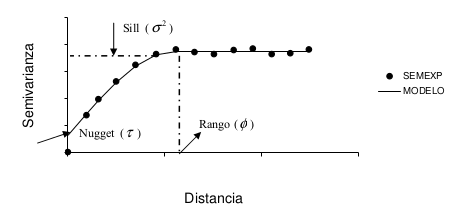
\includegraphics[scale=0.5]{teoria/images/modelo_semivarianza.png}
    \caption{SEMEXP: Semivariograma experimental y MODELO: ajuste de un modelo teórico}
    \label{modelo_semivarianza}
\end{figure}

\begin{itemize}
    \item Nugget($\tau$): Representa una discontinuidad puntual del semivariograma en el origen. Puede ser debido a errores de medición en la variable o a la escala de la misma- En algunas ocasiones puede ser indicativo de que parte de la estructura espacial se concentra a distancias inferiores a las observadas.
    \item Sill($\sigma^2$): Es un estimador de la varianza de las variables del proceso. También puede definirse como el limite del semivariograma cuando la distancia $h$ tiende a infinito
    \item Rango($\phi$) Es términos prácticos corresponde a la distancia a partir de la cual dos observaciones son independientes. El rango se interpreta como la zona de influencia. Existen algunos modelos de semivariograma en los que no existe una distancia finita para la cual dos pbservaciones sean independientes; por ello se llama rango efectivo a la distancia para la cual el semivariograma alcanza el $95\%$ de la meseta (sill) 
\end{itemize}

 Algunos de modelos más comunes y que son presentados por (Armstrong, 1950 )\cite{armstrong} son los siguientes

\subparagraph{Efecto Pepita}

Corresponde a un modelo puramente aleatorio (ruido blanco), donde no existe correlación entre los
valores sin importar la cercanía entre los mismos.

\begin{equation*}
\gamma(h) = 
\left\{ 
\begin{aligned}
0  ,&   h =0\\
C ,& |h| > 0
\end{aligned}
\right.
\end{equation*}

\subparagraph{Modelo esférico}

Es el modelo más utilizado, se compone de una expresión polinómica simple y su forma coincide con
lo observado generalmente; inicialmente un crecimiento casi lineal hasta cierta distancia y luego la
estabilización, alcanzada en un punto cuya abscisa sea $2a\sqrt{3}$

\begin{equation*}
\gamma(h) = 
\left\{ 
\begin{aligned}
C\left( \frac{3|h|}{2a} - \frac{|h|^3}{2a^3}\right) & ,   & |h| > 0\\
C & ,   & |h| > 0
\end{aligned}
\right.
\end{equation*}


\subparagraph{Modelo exponencial}
El rango efectivo de este modelo se encuentra en $a$, al ser la distancia en la cual se alcanza el $95\%$ de su límite; este modelo tiene un comportamiento lineal para distancias pequeñas, en el caso del exponencial inicialmente presenta un crecimiento muy rápido.

\begin{equation*}
\gamma(h) = 
\{C (1- exp(-|h|/a))\}
\end{equation*}

\subparagraph{Modelo Gaussiano}
Representa un fenómeno extremadamente continuo, donde se ha evidenciando la ocurrencia de
inestabilidades numéricas cuando no se hace uso del efecto pepita. Su rango efectivo es $\sqrt{3}a$.


\begin{equation*}
\gamma(h) = 
\{C (1- exp(-|h|^2/a^2))\}
\end{equation*}






